\documentclass[11pt]{article}

\usepackage{report}

\usepackage[utf8]{inputenc} % allow utf-8 input
\usepackage[T1]{fontenc}    % use 8-bit T1 fonts
\usepackage[colorlinks=true, linkcolor=black, citecolor=blue, urlcolor=blue]{hyperref}       % hyperlinks
\usepackage{url}            % simple URL typesetting
\usepackage{booktabs}       % professional-quality tables
\usepackage{amsfonts}       % blackboard math symbols
\usepackage{nicefrac}       % compact symbols for 1/2, etc.
\usepackage{listings}
\usepackage{microtype}      % microtypography
\usepackage{lipsum}		% Can be removed after putting your text content
\usepackage{graphicx}
\graphicspath{ {./images/} }
\usepackage{natbib}
\usepackage{doi}
\setcitestyle{aysep={,}}
\usepackage{array}

\usepackage{xcolor}
\definecolor{codegreen}{rgb}{0,0.6,0}
\definecolor{codegray}{rgb}{0.5,0.5,0.5}
\definecolor{codeorange}{rgb}{1,0.49,0}
\definecolor{backcolour}{rgb}{0.95,0.95,0.96}

\lstdefinestyle{mystyle}{
    backgroundcolor=\color{backcolour},   
    commentstyle=\color{codegray},
    keywordstyle=\color{codeorange},
    numberstyle=\tiny\color{codegray},
    stringstyle=\color{codegreen},
    basicstyle=\ttfamily\footnotesize,
    breakatwhitespace=false,         
    breaklines=true,                 
    captionpos=b,                    
    keepspaces=true,                 
    numbers=left,                    
    numbersep=5pt,                  
    showspaces=false,                
    showstringspaces=false,
    showtabs=false,                  
    tabsize=2,
    xleftmargin=10pt,
}

\lstset{style=mystyle}

\title{CT2109 - Object-Oriented Programming: Data Structures \& Algorithms}

\author{Andrew Hayes\\
\AND
\AND
\AND
\AND
    Student ID: 21321503 \\
\AND
	2BCT\\
\AND
    University of Galway\\
}

% Uncomment to remove the date
% \date{February 2022}

% Uncomment to override  the `A preprint' in the header
\renewcommand{\undertitle}{Assignment 01}
\renewcommand{\headeright}{CT2109 Assignment 01}
\renewcommand{\shorttitle}{}

%%% Add PDF metadata to help others organize their library
%%% Once the PDF is generated, you can check the metadata with
%%% $ pdfinfo template.pdf
% \hypersetup{
% pdftitle={A template for the arxiv style},
% pdfsubject={q-bio.NC, q-bio.QM},
% pdfauthor={David S.~Hippocampus, Elias D.~Striatum},
% pdfkeywords={First keyword, Second keyword, More},
% }

\begin{document}
\maketitle

\newpage
\setcounter{page}{1}
\section{Problem Statement with Analysis \& Design Notes}
At its most basic, this assignment will require an array of all the letters of the alphabet, and two methods: 
one to loop through the array in alphabetical order, and the other to loop it in counter-alphabetical order.

There will be a choice presented to the user whether to loop through the alphabet \textit{forwards} (alphabetical order) 
or \textit{backwards} (counter-alphabetical) order. 
To choose between these two options there will be a case statement. 
A \verb|char| will be scanned in from the user. 
If the \verb|char| is equal to \verb|'f'|, then the \verb|forwards()| method will be executed, and the time taken will be printed out. 
If the \verb|char| is equal to \verb|'b'|, then the \verb|backwards()| method will be executed, and the time taken will be printed out. 
The \verb|default| of the case statement will be to print an error message and exit with code \verb|1|. 
While the use of two separate methods for the alphabetical \& counter-alphabetical versions is not the absolute most efficient option in terms of lines of code, 
the use of separate functions enhances the readability of the code and allows for a cleaner implementation, at the cost of repeating only two or three lines of code. 
It also reduces the need for nested if statements, which are both inefficient and often difficult to read. 

The \verb|forwards()| \& \verb|backwards()| methods will be essentially the same. 
They will both return the \verb|long| data type, which will be the time taken in seconds. 
To calculate the time taken in seconds, before the ``game'' begins, the start time will be recorded with \verb|System.currentTimeMillis()|. 
The end time will be recorded in a similar manner at the end, and the total will be calculated from subtracting one from the other. 
This total will then be divided by 1000 (to convert from milliseconds to seconds) and then returned, where it will then be printed out. 

The game itself will work in a similar manner in both methods: the array of the letters of the alphabet will be looped through using a \verb|while| loop 
A character will be scanned in from the user. 
If the character is correct, a success message will be printed and the index variable incremented or decremented as appropriate for the method. 
Otherwise, the loop will be executed again on the same character, effectively ignoring the input, until the appropriate character is entered. 
If the index is at the last character of either sequence (alphabetical or counter-alphabetical), a special message will be printed out if the answer is correct. 

The only real difference between the two methods will be the way in which they loop through the alphabet array. 
\verb|forwards()| will loop through the array in alphabetical order, starting at index \verb|0| and incrementing the index for each correct answer, with the loop condition \verb|while (i < 26)|. 
\verb|backwards()| will loop the array in counter-alphabetical order, starting at index \verb|25| and decrementing the index for each correct answer, with the loop condition \verb|while (i >= 0)|. 


\section{Code}
\lstinputlisting[language=Java, breaklines=true, caption={Alphabet.java}]{../code/Alphabet.java}

\section{Testing}
There are two main scenarios that must be tested for both the \verb|forwards()| \& \verb|backwards()| methods: correct input \& incorrect input. 
Of these two main scenarios, we should test them at the first character of the sequence, the last character of the sequence, and some of the middle characters. 
The main reason for this is that the first \& last characters are in a sense special, particularly the last one, so what may work for the ``middle'' characters may not work for the others. 

Furthermore, the case statement to choose between forwards \& backwards should be tested with input \verb|f|, \verb|b|, and some incorrect, third option. 

\begin{center}
\begin{figure}[htp]
    \centering
    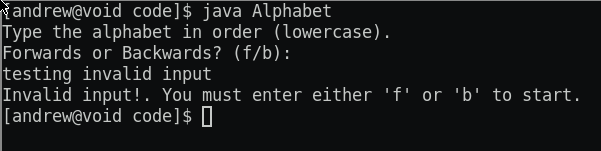
\includegraphics[width=0.7\textwidth]{invalid_input.png}
    \caption{Testing invalid input to the case statement}
\end{figure}
\end{center}

\begin{center}
\begin{figure}[htp]
    \centering
    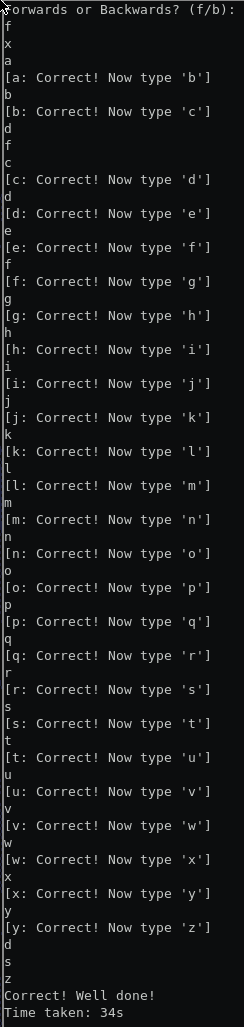
\includegraphics[width=0.3\textwidth]{forwards.png}
    \caption{Testing forwards with valid \& invalid, first, middle, \& last input}
\end{figure}
\end{center}

\begin{center}
\begin{figure}[htp]
    \centering
    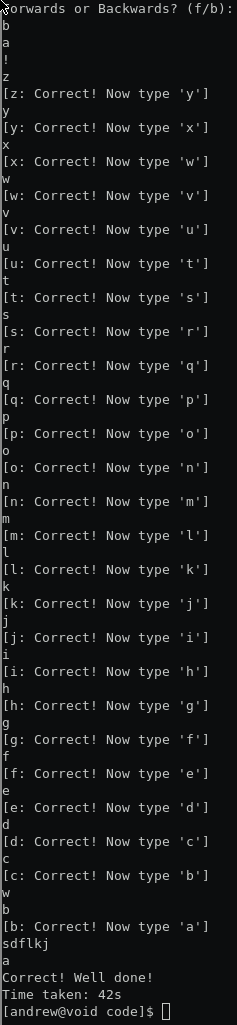
\includegraphics[width=0.3\textwidth]{backwards.png}
    \caption{Testing backwards with valid \& invalid, first, middle, \& last input}
\end{figure}
\end{center}
\end{document}
